% TFM.tex
% TFM
% Daniel Rodríguez Chavarría
% Sevilla, 6 de octubre de 2017
% =============================================================================

\documentclass[a4paper,12pt,twoside]{book}

%%%%%%%%%%%%%%%%%%%%%%%%%%%%%%%%%%%%%%%%%%%%%%%%%%%%%%%%%%%%%%%%%%%%%%%%%%%%%%
%%  Paquetes adicionales                                                   %%
%%%%%%%%%%%%%%%%%%%%%%%%%%%%%%%%%%%%%%%%%%%%%%%%%%%%%%%%%%%%%%%%%%%%%%%%%%%%%%

\usepackage[utf8x]{inputenc}       % Acentos de UTF8
\usepackage[spanish]{babel}        % Castellanización.
\usepackage[T1]{fontenc}           % Codificación T1 con European Computer
                                   % Modern.  
\usepackage{graphicx}
\usepackage{fancyvrb}              % Verbatim extendido
\usepackage{fancyref}              % Referencias extendidas
\usepackage{makeidx}               % Índice
\usepackage{amsmath}               % AMS LaTeX
\usepackage{amsthm} 
\usepackage{amssymb}
%\usepackage{listings}                 %Haskell code
%\usepackage{minted}               %Haskell code
\usepackage{latexsym}
\usepackage[colorinlistoftodos
           , backgroundcolor = yellow
           , textwidth = 4cm
           , shadow
           , spanish]{todonotes}
% Fuentes
\usepackage{mathpazo}              % Fuentes semejante a palatino
\usepackage[scaled=.90]{helvet}
\usepackage{cmtt}
\renewcommand{\ttdefault}{cmtt}
\usepackage{a4wide}
% \usepackage{xmpincl}               % Incluye metadato de licencia CC.

% Tikz
\usepackage{tkz-berge}
\usetikzlibrary{shapes,trees}

% Desactivar <,> cuando se hacen dibujos con tikz.
\tikzset{
every picture/.append style={
  execute at begin picture={\deactivatequoting},
  execute at end picture={\activatequoting}
  }
}

% Márgenes
\usepackage[margin=1in]{geometry}

% Control de espacios en la tabla de contenidos:
\usepackage[titles]{tocloft}
\setlength{\cftbeforechapskip}{2ex}
\setlength{\cftbeforesecskip}{0.5ex}
\setlength{\cftsecnumwidth}{12mm}
\setlength{\cftsubsecindent}{18mm}

% Control de listas
% Elimina espacio entre item y párrafo y coloca item en el margen izquierdo
% \usepackage{enumitem}
% \setlist[enumerate,itemize]{noitemsep, nolistsep, leftmargin=*}

\usepackage{minitoc}

% Doble espacio entre líneas
\usepackage{setspace}
\onehalfspacing


% \linespread{1.05}                % Distancia entre líneas
\setlength{\parindent}{5mm}        % Indentación de comienzo de párrafo
\deactivatetilden                  % Elima uso de ~ para la eñe
\raggedbottom                      % No ajusta los espacios verticales.

\usepackage[%
  pdftex,
  pdfauthor={Daniel R. Chavarria},%
  pdftitle={SAT-pol},%
  pdfstartview=FitH,%
  bookmarks=false,%
  colorlinks=true,%
  urlcolor=blue,%
  unicode=true]{hyperref}      

\usepackage{tikz}

%%%%%%%%%%%%%%%%%%%%%%%%%%%%%%%%%%%%%%%%%%%%%%%%%%%%%%%%%%%%%%%%%%%%%%%%%%%%%%
%%  Cabeceras                                                              %%
%%%%%%%%%%%%%%%%%%%%%%%%%%%%%%%%%%%%%%%%%%%%%%%%%%%%%%%%%%%%%%%%%%%%%%%%%%%%%%

\usepackage{fancyhdr}

\addtolength{\headheight}{\baselineskip}

\pagestyle{fancy}

\cfoot{}

\fancyhead{}
\fancyhead[RE]{\bfseries \nouppercase{\leftmark}}
\fancyhead[LO]{\bfseries \nouppercase{\rightmark}}
\fancyhead[LE,RO]{\bfseries \thepage}

%%%%%%%%%%%%%%%%%%%%%%%%%%%%%%%%%%%%%%%%%%%%%%%%%%%%%%%%%%%%%%%%%%%%%%%%%%%%%%
%%  Definiciones                                                           %%
%%%%%%%%%%%%%%%%%%%%%%%%%%%%%%%%%%%%%%%%%%%%%%%%%%%%%%%%%%%%%%%%%%%%%%%%%%%%%%

\input definiciones
\def\mtctitle{Contenido}

%%%%%%%%%%%%%%%%%%%%%%%%%%%%%%%%%%%%%%%%%%%%%%%%%%%%%%%%%%%%%%%%%%%%%%%%%%%%%%
%%  Título                                                                 %%
%%%%%%%%%%%%%%%%%%%%%%%%%%%%%%%%%%%%%%%%%%%%%%%%%%%%%%%%%%%%%%%%%%%%%%%%%%%%%%

\title{\Huge Título del TFM}
\author{Autor}
\date{\vfill \hrule \vspace*{2mm}
  \begin{tabular}{l}
      \href{http://www.cs.us.es/glc}
           {Grupo de Lógica Computacional} \\
      \href{http://www.cs.us.es}
           {Dpto. de Ciencias de la Computación e Inteligencia Artificial} \\
      \href{http://www.us.es}
           {Universidad de Sevilla}  \\
      Sevilla, \today
  \end{tabular}\hfill\mbox{}}




%%%%%%%%%%%%%%%%%%%%%%%%%%%%%%%%%%%%%%%%%%%%%%%%%%%%%%%%%%%%%%%%%%%%%%%%%%%%%%%
%%  Construcción del índice                                                 %%
%%%%%%%%%%%%%%%%%%%%%%%%%%%%%%%%%%%%%%%%%%%%%%%%%%%%%%%%%%%%%%%%%%%%%%%%%%%%%%%

\makeindex

%%%%%%%%%%%%%%%%%%%%%%%%%%%%%%%%%%%%%%%%%%%%%%%%%%%%%%%%%%%%%%%%%%%%%%%%%%%%%%%
%%  Teoremas y definiciones                                                 %%
%%%%%%%%%%%%%%%%%%%%%%%%%%%%%%%%%%%%%%%%%%%%%%%%%%%%%%%%%%%%%%%%%%%%%%%%%%%%%%%
\theoremstyle{definition}
\newtheorem{thm}{Teorema}[section]
\newtheorem{cor}[thm]{Corolario}
\newtheorem{lem}[thm]{Lema}
\newtheorem{prop}[thm]{Proposición}
\newtheorem{defn}[thm]{Definición}

%%%%%%%%%%%%%%%%%%%%%%%%%%%%%%%%%%%%%%%%%%%%%%%%%%%%%%%%%%%%%%%%%%%%%%%%%%%%%%
%%  Documento                                                              %%
%%%%%%%%%%%%%%%%%%%%%%%%%%%%%%%%%%%%%%%%%%%%%%%%%%%%%%%%%%%%%%%%%%%%%%%%%%%%%%

% \includeonly{Introduccion}

% \includexmp{licencia}

\begin{document}
% \lstset{language=Haskell}
\dominitoc

\begin{titlepage}
 \vspace*{2cm}
  \begin{center}
    {\huge \textbf{Título del TFM}}
  \end{center}
  \vspace{4cm}
  \begin{center}
    \leavevmode
\includegraphics[totalheight=6cm]{sello.png}\\[3cm]
    {\normalsize Facultad de Matemáticas} \\
    {\normalsize Departamento de Ciencias de la Computación e Inteligencia Artificial}\\
    {\normalsize Trabajo Fin de Máster} \\
  \end{center}
  \begin{center}
    {\large \textbf{Autor}}
  \end{center}
  \newpage
 
 \begin{flushright}
   \vspace*{5cm}
   \begin{minipage}{8.45cm}
      Agradecimientos
    \end{minipage}

      \vspace*{7.5mm}

  \end{flushright}
  \vspace*{\fill}

  \newpage


  
  % \begin{flushright}
  \begin{center}
   \vspace*{5cm}
    \begin{minipage}{14cm}
      El presente Trabajo Fin de Máster se ha realizado en el Departamento de
      Ciencias de la Computación e Inteligencia Artificial de la Universidad de
      Sevilla.

      \vspace*{7.5mm}

      Supervisado por
      % \vspace*{5mm}
    \end{minipage}\par
    Tutor
    % \end{flushright}
    \end{center}
  \vspace*{\fill}

  \newpage

  \vspace*{3cm}
  {\huge \textit{Abstract}}

  \vspace{2cm}
  Resumen en inglés
  
\end{titlepage}
\newpage

\noindent
Esta obra está bajo una licencia Reconocimiento--NoComercial--CompartirIgual
2.5 Spain de Creative Commons. 

\vspace*{4ex}

\begin{center}
\fbox{
\begin{minipage}{175mm}
\vspace*{1ex}
\noindent                     
{\bf Se permite:}
\begin{itemize}                         
\item copiar, distribuir y comunicar públicamente la obra
\item hacer obras derivadas
\end{itemize}
         
\noindent       
{\bf Bajo las condiciones siguientes:}

\begin{minipage}[t]{20mm}
  \vspace*{0mm}\hspace*{1em}
  
\includegraphics[scale=0.35]{licencia/deed.png}
\end{minipage}%
\begin{minipage}[t]{15cm}
  \vspace*{0mm}
  {\bf Reconocimiento}. Debe reconocer los créditos de la  obra de la manera
  especificada por el autor.  
\end{minipage}
\\[1ex]

\begin{minipage}[t]{20mm}
  \vspace*{0mm}\hspace*{1em}
  
\includegraphics[scale=0.35]{licencia/deed-eu.png}
\end{minipage}%
\begin{minipage}[t]{15cm}
  \vspace*{2mm}
  {\bf No comercial}. No puede utilizar esta obra para fines comerciales.
\end{minipage}
\\[1ex]

\begin{minipage}[t]{20mm}
  \vspace*{0mm}\hspace*{1em}
  
\includegraphics[scale=0.35]{licencia/deed_002.png}
\end{minipage}%
\begin{minipage}[t]{15cm}
  \vspace*{-2mm}
  {\bf Compartir bajo la misma licencia}. Si altera o transforma esta obra, o
  genera una obra derivada, sólo puede distribuir la obra generada bajo una
  licencia idéntica a ésta. 
\end{minipage}

\begin{itemize}    
\item Al reutilizar o distribuir la obra, tiene que dejar bien claro los
  términos de la licencia de esta obra. 
\item Alguna de estas condiciones puede no aplicarse si se obtiene el permiso
 del titular de los derechos de autor.
\end{itemize}
\vspace*{1ex}
\end{minipage}}
\end{center}

\vspace*{4ex}

Esto es un resumen del texto legal (la licencia completa). Para ver una copia
de esta licencia, visite 
\href{http://creativecommons.org/licenses/by-nc-sa/2.5/es/}
     {\url{http://creativecommons.org/licenses/by-nc-sa/2.5/es/}}
o envie una carta a Creative Commons, 559 Nathan Abbott Way, Stanford,
California 94305, USA.

%%% Local Variables: 
%%% mode: latex
%%% TeX-master: t
%%% End: 

\newpage 

\tableofcontents
\newpage

\addcontentsline{toc}{chapter}{Introducción}
\chapter*{Introducción}


\hfil \textit{El lenguaje de la verdad debe ser, sin duda alguna, simple y sin artificios}

\hfil \hfil \hfil \hfil Séneca\\\\


La lógica proposicional nos permite representar el conocimiento de manera que sea sencillo trabajar con él, pero a la vez plantea un marco de estudio de gran interés y con multitud de aplicaciones. Uno de los problemas centrales de la lógica es el problema de satisfacibilidad, es decir, preguntarse si existe algún mundo en el que un conjunto de hechos o propiedades sean posibles.\\

Antes de continuar, se pondrá al lector en situación dando una descripción detallada del problema de satisfacibilidad booleana; así como de su importancia, tanto para la comunidad científica internacional como para la sociedad en general.

\section{El problema $SAT$}

%\subsection{Definición}
Tal y como se define en la página \pageref{def:sat}, una fórmula proposicional $F$ se dice \textit{satisfacible} si existe al menos una interpretación $i$ de $F$ que sea modelo de la fórmula. A partir de esta definición, es natural preguntarse cuándo una formula dada es satisfacible o no. \\ 

Éste es el problema de la satisfacibilidad booleana o el comúnmente conocido como problema $SAT$. En definitiva consiste en saber si existe alguna forma de sustituir las variables proposicionales por $True$ o $False$, de manera que la fórmula sea verdadera. \\

Es importante destacar que para una fórmula con 10 variables, existen $2^{10} = 1024$ valoraciones a comprobar. Si a esto se suma que para que una fórmula se considere ``mínimamente interesante'' (en el mundo empresarial, por ejemplo) debe tener cientos de variables; el orden de magnitud de comprobaciones que se han de hacer es similar al número de átomos que hay en el universo. Este crecimiento tan rápido de combinaciones se debe a la complejidad exponencial intrínseca al problema de satisfacibilidad. \\

En teoría de la complejidad computacional, es considerado el problema capital de la clase de complejidad $NP$ al ser también un problema $NP$ duro ($NP$-hard), y ganándose así el estatus de problema $NP$-completo. \\

Respecto a los problemas $NP$-completos, no hay manera eficiente conocida de obtener una solución. Es decir, el tiempo requerido para resolver el problema usando cualquier algoritmo conocido aumenta muy rápidamente a medida que el tamaño del problema crece.\\

Como consecuencia, el problema de determinar si es posible resolver estos problemas de forma rápida, llamado problema $P$ versus $NP$ (¿$P=NP$?), es uno de los principales problemas sin resolver de la matemática e informática actuales. Es por esto que en el año 2000, el \textit{Clay Mathematics Institute} lo declaró como el primer problema del milenio, junto a otros siete. Este título no es en vano, ya que se cree que estos problemas marcarán el devenir de la comunidad científico-matemática.\\

Para comprender algo mejor la importancia del problema ¿$P=NP$? es importante conocer las consecuencias de su resolución. Si resultara que no son iguales, el impacto en la sociedad sería mínimo ya que únicamente se dejarían de buscar algoritmos de complejidad polinomial para resolver problemas de la clase $NP$.\\

Sin embargo, si se demostrase que ambas clases de complejidad son iguales, las implicaciones para la sociedad actual serían de una magnitud incomparable. Esto se debe a que la robustez de los sistemas criptográficos actuales se basan en la intratabilidad de ciertos problemas de la clase $NP$. Si éstos fueran resolubles en tiempo polinomial peligrarían todas las comunicaciones y las claves bancarias dejarían de ser seguras. Por otro lado, no todas las consecuencias son negativas ya que multitud de problemas de ámbito empresarial o social serían tratables; y por tanto, los costes se reducirían y los beneficios aumentarían.\\

Aunque, una vez vista la importancia del problema ¿$P=NP$? es natural preguntarse cómo podría resolverse. La respuesta es tan sencilla como dar un algoritmo que trabaje en tiempo polinomial en función del dato de entrada para un problema $NP$-completo, o demostrar que no existe dicho algoritmo. \\ 

El problema $NP$-completo objeto de la mayoría de estudios por parte de la comunidad científica es el problema $SAT$. Es tal su popularidad que cada año se publican multitud de nuevos algoritmos que dicen mejorar la eficiencia de resolución, y que se basan en las técnicas informáticas más innovadoras. \\

Con el objetivo de regular dicha competición, así como de identificar y promover nuevos retos relacionados con la resolución del problema $SAT$ surge la \textit{SAT Competition 2002}\footnote{\url{http://www.satcompetition.org/2002/}} \footnote{\url{http://www.satcompetition.org}}, enmarcada dentro del \textit{Fifth  International Symposium on the Theory and Applications of Satisfiability Testing} \footnote{\url{http://gauss.ececs.uc.edu/Conferences/SAT2002/}}. Y desde ese año, de forma anual o bianual, se celebra tal competición. \\

Para poder participar en dicha competición se debe seguir un estándar, cuya regla principal es que la fórmula (o base de conocimiento) de entrada está escrita en un fichero de texto en forma normal conjuntiva utilizando el formato $DIMACS$ \footnote{\url{http://www.satcompetition.org/2009/format-benchmarks2009.html}}, que se describirá con detalle más adelante.

Enmarcando el trabajo aquí presente en el contexto actual, éste pretende sentar las bases de un algoritmo que resuelva el problema $SAT$, para posteriormente implementar una herramienta eficiente en lenguaje Haskell \footnote{\url{https://www.haskell.org}} que cumpla los estándares de dicha competición.\\

%%%%%%%%%%%%%%%%%%%%%%%%%%%%%%%%%

\section{Gestión del proyecto}
Es comúnmente aceptado que el proceso de creación de un programa consta de 5 etapas principales:

\begin{enumerate}
\item El desarrollo lógico del programa para resolver un problema en particular.
\item Escritura de la lógica del programa empleando un lenguaje de programación específico (codificación del programa).
\item Ensamblaje o compilación del programa hasta convertirlo en lenguaje de máquina.
\item Prueba y depuración del programa.
\item Desarrollo de la documentación.
\end{enumerate}

En esta sección se tratarán las tecnologías auxiliares usadas en las distintas etapas a fin de comprender su importancia dentro del proyecto, así como la necesidad de usar las herramientas que están a disposición del programador para desarrollar una aplicación de mayor calidad en menor tiempo.\\

El lenguaje de programación escogido es el lenguaje funcional Haskell, ya que encaja perfectamente con las necesidades del proyecto. Según la propia página web de Haskell, es un lenguaje que combina un fuerte sistema de tipos, inferencia de tipos y código de alto nivel, lo que afirman que ofrece al usuario la velocidad de desarrollo de lenguajes como Python o Ruby, además de una mayor robustez que lenguajes como Java o C++ .\\

A esto se le debe añadir que goza de una comunidad muy activa y un ecosistema de librerías muy rico, con multitud de librerías centradas en las matemáticas, y por ende, en los polinomios. Además, al ser objetivo del proyecto el definir diversas funciones matemáticas que actúen sobre el cuerpo $\mathbb{F} [\textbf{x}]$, resulta natural escoger un lenguaje funcional tipado.\\

En lo que refiere a la tercera etapa, destacar la herramienta \texttt{stack}\footnote{\url{https://docs.haskellstack.org/en/stable/README/}} que, definiendo una jerarquía específica de ficheros en nuestro proyecto, asiste el ensamblado y compilación. Esto permite usar el programa en cualquier computador sin la necesidad de instalar librerías auxiliares ya que con tener instalado \texttt{stack} es suficiente. Aunque a la postre, el compilador primario que usa Haskell es GHC (Glasgow Haskell Compiler \footnote{\url{https://www.haskell.org/ghc/}}), un compilador en la vanguardia tecnológica, y de código libre, diseñado específicamente para Haskell.\\

Para la comprobación de la aplicación, el sistema de tipos de Haskell garantiza una cierta robustez, y es que asegura que cada función se utilice sobre los tipos para los que está diseñada. Por ejemplo, si intentamos calcular la suma de dos caracteres se devolverá un error al compilar.\\

Otro detalle a destacar de \texttt{stack} es que está diseñado de forma que la comprobación de los ejemplos sea muy natural y se haga automáticamente al compilar, con ayuda de la librería \texttt{doctest} \footnote{\url{https://hackage.haskell.org/package/doctest}}. Cada vez que en el código hay ($>>>$) se ejecuta lo escrito a continuación y se corrobora si devuelve lo que aparezca en la línea siguiente (si es que se devolviese algo). 

\newpage

Por ejemplo, en

\begin{code}
-- | 
-- >>> 2+2
-- 4
\end{code}

se comprueba si 2+2 devuelve 4. Notar que esto concede al proyecto de mucha robustez frente a modificaciones. Es decir, si se cambia el código de cierta función $f$ buscando una mayor eficiencia pero se comete algún error, se puede detectar al hacer las comprobaciones de los casos base, tanto de esta función como de alguna otra en la que intervenga $f$.\\

Otra ventaja, relacionada con las comprobaciones, que ofrece el lenguaje Haskell es la posibilidad de implementar propiedades matemáticas de las funciones o los tipos. Estas propiedades pueden ser esenciales en el desarrollo teórico pues pueden justificar, por ejemplo, la corrección de la aplicación o parte de ella.\\

Por lo tanto, es parte fundamental del proyecto verificar dichas propiedades mediante la librería \texttt{quickCheck} \footnote{\url{https://hackage.haskell.org/package/QuickCheck}}. Esta librería manda ejecutar 100 ejemplos y casos límites (el número 0, listas vacías, etc) para ver si sobre ellos se sigue verificando la propiedad. En el proyecto se comprobarán estas propiedades cada vez que se compile ya que junto a cada propiedad $prop$ se ha incluido:

\begin{code}
-- | 
-- >>> quickCheck prop
--  +++ OK, passed 100 tests
\end{code}

Así que, si en algún momento del desarrollo se deja de cumplir dicha propiedad para alguna instancia, el sistema devuelve el error.\\

En la etapa de documentación se ha utilizado una versión modificada del lenguaje Haskell, llamada Haskell literario \footnote{\url{https://wiki.haskell.org/Literate_programming}}. Ésta permite escribir código \LaTeX en el mismo archivo en el que se escribe el código Haskell. Por ejemplo, si se escribe en el archivo \texttt{.lhs}:

\begin{codigo}
Es un ejemplo
\begin{code}
ejemplo = "helloworld"
\end{code}
\end{codigo}

Al compilar se verá lo siguiente en el pdf:\\

Es un ejemplo
\begin{code}
ejemplo = "helloworld"
\end{code}

Con la ventaja principal de que la función $ejemplo$ se puede utilizar normalmente, como si se hubiese escrito en un archivo \texttt{.hs} típico.\\

Por último, se ha utilizado la herramienta \texttt{git}\footnote{\url{https://git-scm.com}} de control de versiones, que junto a la plataforma \texttt{GitHub} \footnote{\url{https://github.com}} ha sido de gran ayuda en la depuración del código y la búsqueda de eficiencia.

%%%%%%%%%%%%%%%%%%%%%%%%%%%%%%%%%%

\section{Estructura de la memoria}

%El algoritmo aquí descrito transforma las fórmulas proposicionales en polinomios sobre el cuerpo $\mathbb{F}_2$, de forma que dada una valoración, una fórmula será verdadera (o falsa) si y sólo si el polinomio que le corresponde vale 1 (ó 0) según cierta sustitución. \\

En el primer capítulo, llamado \textit{Interpretación algebraica de la lógica}, se definen formalmente multitud de conceptos lógicos de gran importancia para comprender el funcionamiento de la herramienta. Destacando, la idea de retracción conservativa de una base de conocimiento, que consiste en renombrar las fórmulas de entrada usando un lenguaje menor.\\ 

Además, se define e implementa el anillo $\mathbb{F}_2[\textbf{x}]$ mediante la librería \texttt{HaskellForMaths} \footnote{\url{https://hackage.haskell.org/package/HaskellForMaths}}, optimizada para realizar cálculos como la multiplicación polinomial o la búsqueda de variables.\\ 

La última sección del primer capítulo describe la transformación entre fórmulas lógicas y polinomio. Ésta hace corresponder a cada fórmulas proposicional un polinomio sobre el cuerpo $\mathbb{F}_2$, de forma que dada una valoración, la fórmula será verdadera (o falsa) si y sólo si el polinomio que le corresponde vale 1 (ó 0) según cierta sustitución. Y, posteriormente, sumerge dicho polinomio en el anillo cociente $\mathbb{F}_2[\textbf{x}] /_{\mathbb{I}}$, de forma que sea más fácil trabajar con él.\\

 También se define una función inversa por equivalencias, es decir, si se transforma una fórmula en polinomio, y después otra vez en fórmula; la fórmula obtenida será lógicamente equivalente a la original (pero no tiene que ser igual).\\

En el segundo capítulo se define el concepto de operador de omisión, que transforma una base de conocimiento en otra con una variable proposicional menos, probando que dichos operadores inducen una retracción conservativa. También se prueba que, mediante la aplicación sucesiva del mismo, se puede, en un número finito de pasos, saturar un conjunto de fórmulas proposicionales en $\top$ ó $\bot$. En caso de obtenerse el primero se dice que el conjunto de fórmulas original es satisfacible, mientras que será insatisfacible en caso contrario.\\

El operador de omisión que se escoge se conoce como regla de independencia y se inspira en un cálculo sobre los polinomios de $\mathbb{F}_2[\textbf{x}] /_{\mathbb{I}}$, haciendo uso de la derivada polinomial (también implementada en esta sección). Con este procedimiento, se traduce el problema de satisfacibilidad a un cálculo polinomial.\\

En el capítulo tercero se expone la herramienta desarrollada, enmarcándola en una competición $SAT$. Previamente, se analizan la importancia del problema de satisfacibilidad así como las tecnologías usadas en el proyecto.

\newpage

 La herramienta se divide principalmente en dos etapas: 

\begin{enumerate}
\item Preprocesado del fichero de entrada en formato \texttt{DIMACS}.
\item Saturación del conjunto de polinomios.
\end{enumerate}

En la última sección del capítulo se analiza la herramienta mediante diversas instancias organizadas en orden de complejidad en tres ficheros (\texttt{easy}, \texttt{medium} y \texttt{hard}). Fruto de dicho análisis se detecta e implementa una mejora: la introducción de una heurística a la hora de escoger el orden en el que se van a olvidar las variables.\\

En resumen, con ayuda de las matemáticas damos respuesta al problema de satisfacibilidad, clave en la lógica proposicional. De esta forma obtenemos una respuesta matemática en la búqueda de la verdad, un paso a tener en cuenta, ya que, tal y como decía \textit{Lemoine}:

\begin{center}
\textit{Una verdad matemática no es ni simple ni complicada en si misma, es una verdad}\\
\hspace{10.7cm} Émile Lemoine
\end{center}
\chapter{Interpretación algebraica de la lógica}\label{sec:interp}

En este capítulo se estudiarán las principales relaciones entre la lógica proposicional y los 
polinomios con coeficientes en cuerpos finitos, centrando la atención en $\mathbb{F}_2$, 
el cuerpo finito con dos elementos.\\

La idea principal que subyace en la interpretación algebraica de la lógica es la de hacerle corresponder a cada fórmula un polinomio de forma que la función valor de verdad inducida por la fórmula se pueda entender como una función polinomial de $\mathbb{F}_2$. En otras palabras, se persigue que si la fórmula es verdadera, el valor del polinomio que tiene asociado es 1; mientras que si la fórmula es falsa, el polinomio vale 0.\\

En la Figura \ref{fig:esquema} (abajo) se muestra una representación gráfica de la relación entre las fórmulas proposicionales y los polinomios de $\mathbb{F}_2[x]$. Destacar que se usa el ideal $\mathbb{I}_2 :=(x_1+x_1^2,...,x_n+x_n^2)\subseteq\mathbb{F}_2[x]$ y que $proj$ es la proyección natural sobre el anillo cociente.

\vspace{0.5cm}
\begin{figure}[h]
	\centering
		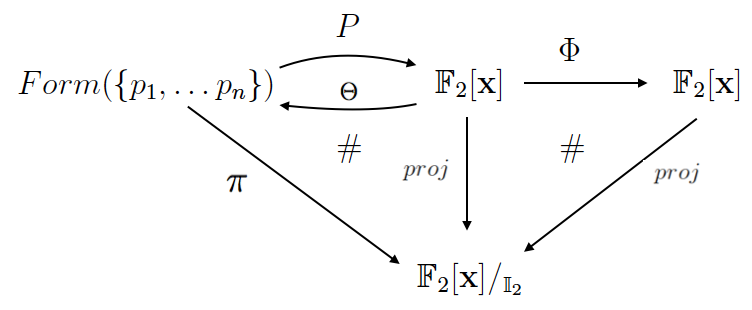
\includegraphics[scale=0.46]{imagenes/conmu.png}
	\caption{Relación entre las fórmulas proposicionales y $\mathbb{F}[x]_2$}
	\label{fig:esquema}
\end{figure}
\vspace{0.5cm}

Destacar que se paralelizará la exposición de la teoría y el desarrollo de las implementaciones en Haskell. Teniendo en cuenta que el objetivo principal de dichos programas es la obtención de una herramienta eficiente para resolver el problema SAT, tema que se tratará con más detalle en los próximos capítulos.
 
\entrada{Logica}
\entrada{Haskell4Maths}
\entrada{F2}
\entrada{Transformaciones}
\chapter{Regla de independencia y prueba no clausal de teoremas}\label{sec:progfunHas}

En este capítulo se hace una breve introducción a la programación funcional en
Haskell suficiente para entender su aplicación en los siguientes
capítulos. Para una introducción más amplia se pueden consultar los apuntes de
la asignatura de Informática de 1º del Grado en Matemáticas
(\cite{Alonso-15b}). 

El contenido de este capítulo se encuentra en el módulo \texttt{PFH} 
\entrada{PFH}.

%%% Local Variables:
%%% mode: latex
%%% TeX-master: "TFG"
%%% End:

\chapter{Aplicaciones}\label{sec:progfunHas}

En este capítulo se hace una breve introducción a la programación funcional en
Haskell suficiente para entender su aplicación en los siguientes
capítulos. Para una introducción más amplia se pueden consultar los apuntes de
la asignatura de Informática de 1º del Grado en Matemáticas
(\cite{Alonso-15b}). 

El contenido de este capítulo se encuentra en el módulo \texttt{PFH} 
\entrada{PFH}.

%%% Local Variables:
%%% mode: latex
%%% TeX-master: "TFG"
%%% End:

\addcontentsline{toc}{chapter}{Conclusión}
\chapter*{Conclusión}

\hfil \textit{La lógica es el principio de la sabiduría, no el final.}

\hfil \hfil \hfil Leonard Nimoy \\\\

La interpretación algebraica de la lógica proposicional representa una valioso recurso que nos permite aplicar técnicas algebraicas a la representación del conocimiento y el razonamiento. En este trabajo se presenta un modelo algebraico para resolver problemas cuyo conocimiento se representa mediante fórmulas de la lógica proposicional.\\

La estructura del trabajo es la natural; es decir, en el primer capítulo se establecen las bases teóricas y los fundamentos necesarios; en el segundo capítulo se presenta el modelo lógico-algebraico, probando su robustez y completitud refutacional; mientras que en el tercer y último capítulo se describe la implementación del algoritmo en el lenguaje Haskell.\\

Destacar que las aplicaciones del modelo aquí presentado son muy variados, ya que no sólo es útil para resolver el problema de satisfacibilidad booleana, sino que también para la detección de estados peligrosos o la descomposición de bases de conocimiento, por ejemplo.\\

Como trabajos futuros destacan tres líneas principales de investigación:

\begin{itemize}
\item[•] Tratar de mejorar la eficiencia de la implementación.
\item[•] Extender el modelo a lógicas multi-valuadas.
\item[•] Dar de forma explícita el algoritmo formal, estudiando su complejidad computacional.
\end{itemize}

\newpage
En la primera línea existen numerosas modificaciones, pero principalmente hacer notar las siguientes:

\begin{enumerate}
\item Desarrollar una librería de polinomios optimizada para calcular la regla de independencia en $\mathbb{F}_2[\textbf{x}]/_{\mathbb{I}}$.
\item Tratar de encontrar alguna propiedad que permita reducir el número de polinomios de una base de conocimiento, ya que, el principal problema detectado es de espacio computacional.
\item Profundizar en el estudio de heurísticas a fin de encontrar una que se adecúe mejor al problema, por ejemplo, ayundándonos del aprendizaje automático.
\item Trata de implementar la paralelización, por ejemplo, mediante el cálculo de la regla de independencia de conjuntos con variables disjuntas. 
\item Debido a que encuentra inconsistencias de forma eficiente, se podría combinar este método con otros más eficientes a la hora de reponder afirmativamente al problema de satisfacibilidad, por ejemplo, con métodos que tratan de encontrar una valoración que haga verdaderas las fórmulas de la base de conocimiento.
\end{enumerate}

%%%%%%%%%%%%%%%%%%%%%%%%%%%%%%%%%%%%%%%%%%%%%%%%%%%%%%%%%%%%%%%%%%%%%%%%%%%%%%% 
%%  Bibliografía                                                            %%
%%%%%%%%%%%%%%%%%%%%%%%%%%%%%%%%%%%%%%%%%%%%%%%%%%%%%%%%%%%%%%%%%%%%%%%%%%%%%%%

\addcontentsline{toc}{chapter}{Bibliografía}
\bibliographystyle{abbrv}
\bibliography{TFG}

%%%%%%%%%%%%%%%%%%%%%%%%%%%%%%%%%%%%%%%%%%%%%%%%%%%%%%%%%%%%%%%%%%%%%%%%%%%%%%%
%%  Índice                                                                  %%
%%%%%%%%%%%%%%%%%%%%%%%%%%%%%%%%%%%%%%%%%%%%%%%%%%%%%%%%%%%%%%%%%%%%%%%%%%%%%%%

\addcontentsline{toc}{chapter}{Indice de definiciones}

\printindex

%%%%%%%%%%%%%%%%%%%%%%%%%%%%%%%%%%%%%%%%%%%%%%%%%%%%%%%%%%%%%%%%%%%%%%%%%%%%%%%
%% § Pendientes                                                              %%
%%%%%%%%%%%%%%%%%%%%%%%%%%%%%%%%%%%%%%%%%%%%%%%%%%%%%%%%%%%%%%%%%%%%%%%%%%%%%%%

%\todototoc
%\listoftodos

\end{document}


%%% Local Variables:
%%% mode: latex
%%% TeX-master: t
%%% End:
